\documentclass{article} \usepackage{graphicx} \graphicspath{ {./tmp_charts} } \usepackage[utf8]{inputenc} \usepackage{polski} \author{C and bash} \title{Równiania} \begin{document} 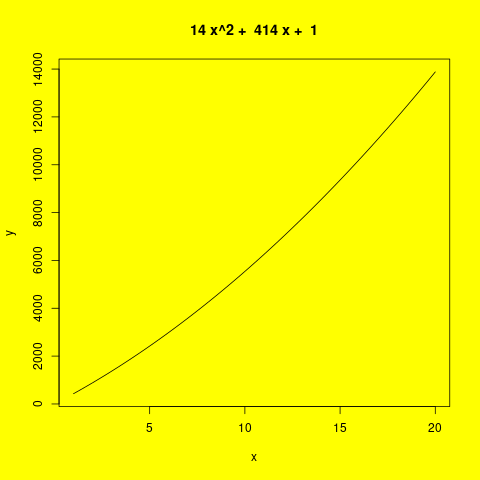
\includegraphics{output.png} \maketitle

\\\
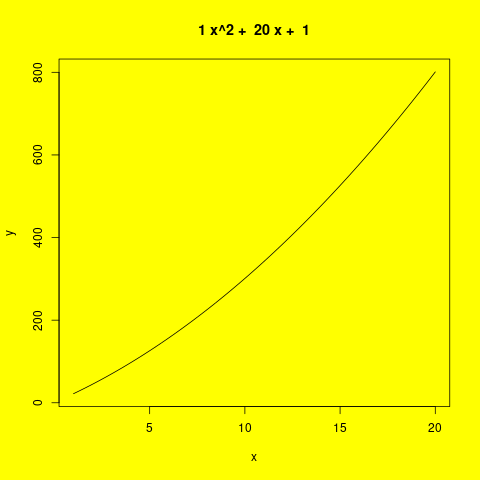
\includegraphics[width=0.5\textwidth]{charts_tmp/0img.png}
\newline 97608314 nanoseconds elpased
\clearpage 

\\\
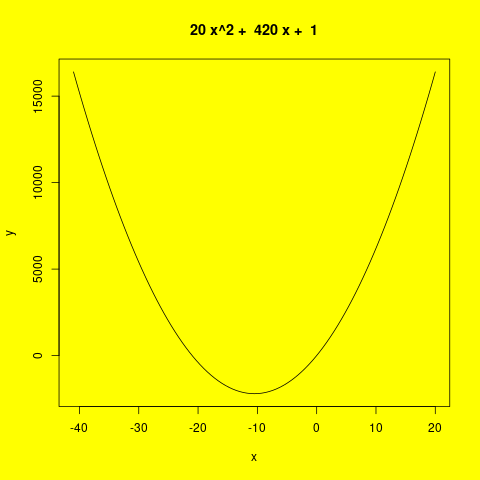
\includegraphics[width=0.5\textwidth]{charts_tmp/1img.png}
\newline 88533490 nanoseconds elpased
\clearpage 

\\\
\includegraphics[width=0.5\textwidth]{charts_tmp/2img.png}
\newline 87078511 nanoseconds elpased
\clearpage 

\\\
\includegraphics[width=0.5\textwidth]{charts_tmp/3img.png}
\newline 85959041 nanoseconds elpased
\clearpage 

\\\
\includegraphics[width=0.5\textwidth]{charts_tmp/4img.png}
\newline 89397537 nanoseconds elpased
\clearpage 
\newline 89397537 nanoseconds elpased for entire script
\end{document}
